%
% 62-rechnen.tex -- Rechnen mit Darstellungen
%
% (c) 2022 Prof Dr Andreas Müller, OST Ostschweizer Fachhochschule
%

%
% Rechnen mit Darstellungen
%
\subsection{Rechnen mit Darstellungen
\label{buch:gruppen:darstellungen:subsection:rechnen-mit-darstellungen}}
Mit Darstellungen kann man rechnen im folgenden Sinn.
Seien
$\varrho_1\colon G\to\operatorname{GL}_{n_1}(\mathbb{R})$
und
$\varrho_2\colon G\to\operatorname{GL}_{n_2}(\mathbb{R})$
Darstellungen der Gruppe $G$.
Dann kann man eine neue, $n_1+n_2$-dimensionale Darstellung konstruieren,
indem man aus den Matrizen $\varrho_1(g)$ und $\varrho_2(g)$ die
Blockmatrix
\begin{equation}
\varrho(g)
=
(\varrho_1\oplus \varrho_2)(g)
=
\left(\raisebox{-1.15cm}{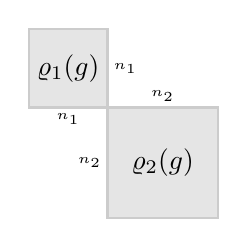
\begin{tikzpicture}[>=latex,thick]
\fill[color=white] (-1.2,-1.2) rectangle (1.2,1.2);
\fill[color=gray!20] (-1.2,1.2) rectangle (-0.2,0.2);
\draw[color=gray!40] (-1.2,1.2) rectangle (-0.2,0.2);
\node at (-0.7,0.25) [below] {\tiny $n_1$};
\node at (-0.25,0.7) [right] {\tiny $n_1$};
\node at (-0.7,0.7) {$\varrho_1(g)\mathstrut$};
\fill[color=gray!20] (-0.2,0.2) rectangle (1.2,-1.2);
\draw[color=gray!40] (-0.2,0.2) rectangle (1.2,-1.2);
\node at (0.5,-0.5) {$\varrho_2(g)\mathstrut$};
\node at (0.5,0.15) [above] {\tiny $n_2$};
\node at (-0.15,-0.5) [left] {\tiny $n_2$};
\end{tikzpicture}}\right).
\label{buch:gruppen:darstellungen:eqn:dirsummatrix}
\end{equation}
Diese Darstellung heisst die {\em direkte Summe} der Darstellungen
$\varrho_1$ und $\varrho_2$.
Für eine natürlich Zahl $k$ soll die
Schreibweise $k\cdot \varrho_1$ als die $k$-fache direkte Summe der
Darstellung $\varrho_1$ interpretiert werden.

